\section{Introduction}\label{sec:intro}
Text-based program editors are flexible and powerful user interfaces, 
so it is little wonder that they remain dominant decades after the teletype.
However, textual user interfaces are not the best tool for every computational job.
% In particular, there are countless 
% data types for which a non-textual
% user interface may situationally be more appropriate.

Consider, as a simple example, a record type
classifying RGBA-encoded colors. 
It is possible to select a particular color by entering
an expression of this type in a text editor, e.g. \li{\{ r: 57, g: 107, b: 57, a: 92 \}}. 
The problem with this \emph{de facto} textual user interface for color selection is that 
it offers no live feedback about which color has been expressed 
and limited editing affordances for choosing a different color.
Analagous critiques apply to strictly textual user interfaces for 
countless other data structures,
e.g. vector graphics,
animation parameters,
musical sequences,
audio filters,
board game states, 
GUI widgets and layouts,
tabular numeric data, 
plots,
geospatial data, 
neural network diagrams, 
biological neuron models, 
and mathematical diagrams.

Practitioners in domains where manipulating data of types like these is 
a central activity 
have largely eschewed general-purpose programming environments 
in favor of specialized graphical end-user applications, e.g. %
image and video editors, music composition software, level design tools, 
and bespoke GUIs written by students or lab technicians.
This is in large part because these applications 
take seriously the need for live feedback, domain-specific 
non-textual data representations, and 
direct manipulation affordances, 
e.g. color palettes, visual timelines, plots, and maps.

The tragedy is that these applications have 
limited support for abstraction and composition.
It is difficult, for example, to bind a
color to a variable for use in multiple locations in an
otherwise directly constructed game map, 
or to define functional combinators to compute portions of an 
otherwise directly constructed musical composition. 
Some applications include \emph{ad hoc} abstraction mechanisms for 
the most common such use cases, e.g. named color swatches, 
but users cannot themselves define new affordances, either programmatic or graphical, 
nor compose
affordances in ways that the application developer did not anticipate.
For example, 
users cannot make even simple changes like replacing a 
numeric text box with a slider,
much less more ambitious changes like importing an alternative 
visual interface for expressing geospatial data queries 
into a civic database front-end. 
% In short, end users and programmers speak entirely different languages, 
% leaving end users to rely helplessly on programmers, 
% and programmers unable to bring their skills to bear 
% when using end-user applications.

% Better support for manipulating data of types like these would be particularly helpful for users engaging in
% live and exploratory programming in domains like web design, media production,
% and data analysis. Indeed, 

This paper aims to bridge the gap between
programmatic and direct manipulation user interfaces by designing 
a programming environment that
is able to surface a GUI when entering an expression of a type for which
it is useful, while retaining full support for symbolic program manipulation
and the abstraction and composition mechanisms
available in modern general-purpose languages, both   
in the spaces between these GUIs and compositionally within these GUIs.

\subsection{Background}\label{sec:background}
\definecolor{mygray}{rgb}{0.93, 0.93, 0.93}
\definecolor{shadecolor}{named}{mygray}

\begin{figure*}
  \begin{minipage}[t]{0.37\textwidth}
    \begin{subfigure}[t]{\linewidth}
    \begin{snugshade}
      \vspace*{-2mm}
      \caption{\textbf{Prior Work:} Graphite \cite{Graphite}}
       \label{fig:graphite}
      \vspace*{1mm}
     \end{snugshade}
      \vspace*{-1mm}
      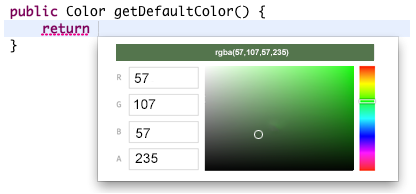
\includegraphics[width=\linewidth]{graphite-color-palette-green.png}
      \vspace*{-5mm}
    \end{subfigure}
    \hspace{8mm}
    \begin{subfigure}[t]{\linewidth}
     \begin{snugshade}
      \vspace*{-2mm}
      \caption{\textbf{This Paper:} Livelits are live and compositional}
    \label{fig:color}
      \vspace*{1mm}
     \end{snugshade}
      \vspace*{-1mm}
      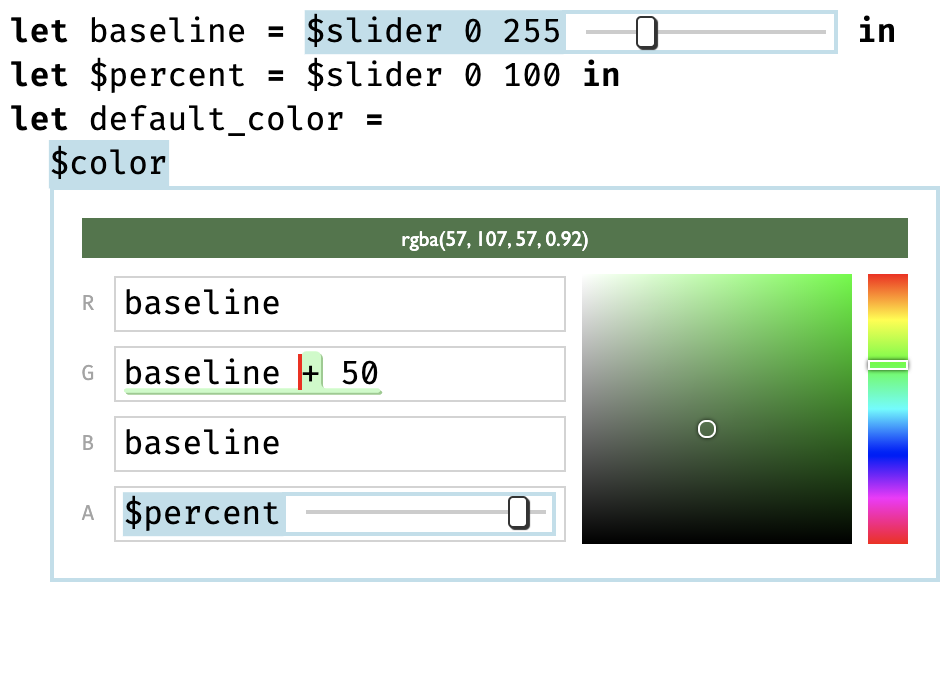
\includegraphics[width=\linewidth]{slider-color-livelits.png}
    \end{subfigure}
  \end{minipage}
  \hspace{10.5mm}
  \begin{subfigure}[t]{0.50\textwidth}
  \begin{snugshade}
   \vspace*{-2mm}
    \caption{\textbf{Case Study}: Grading with Livelits}
    \label{fig:grading}
    \vspace*{1mm}
     \end{snugshade}
    \vspace*{-1mm}
    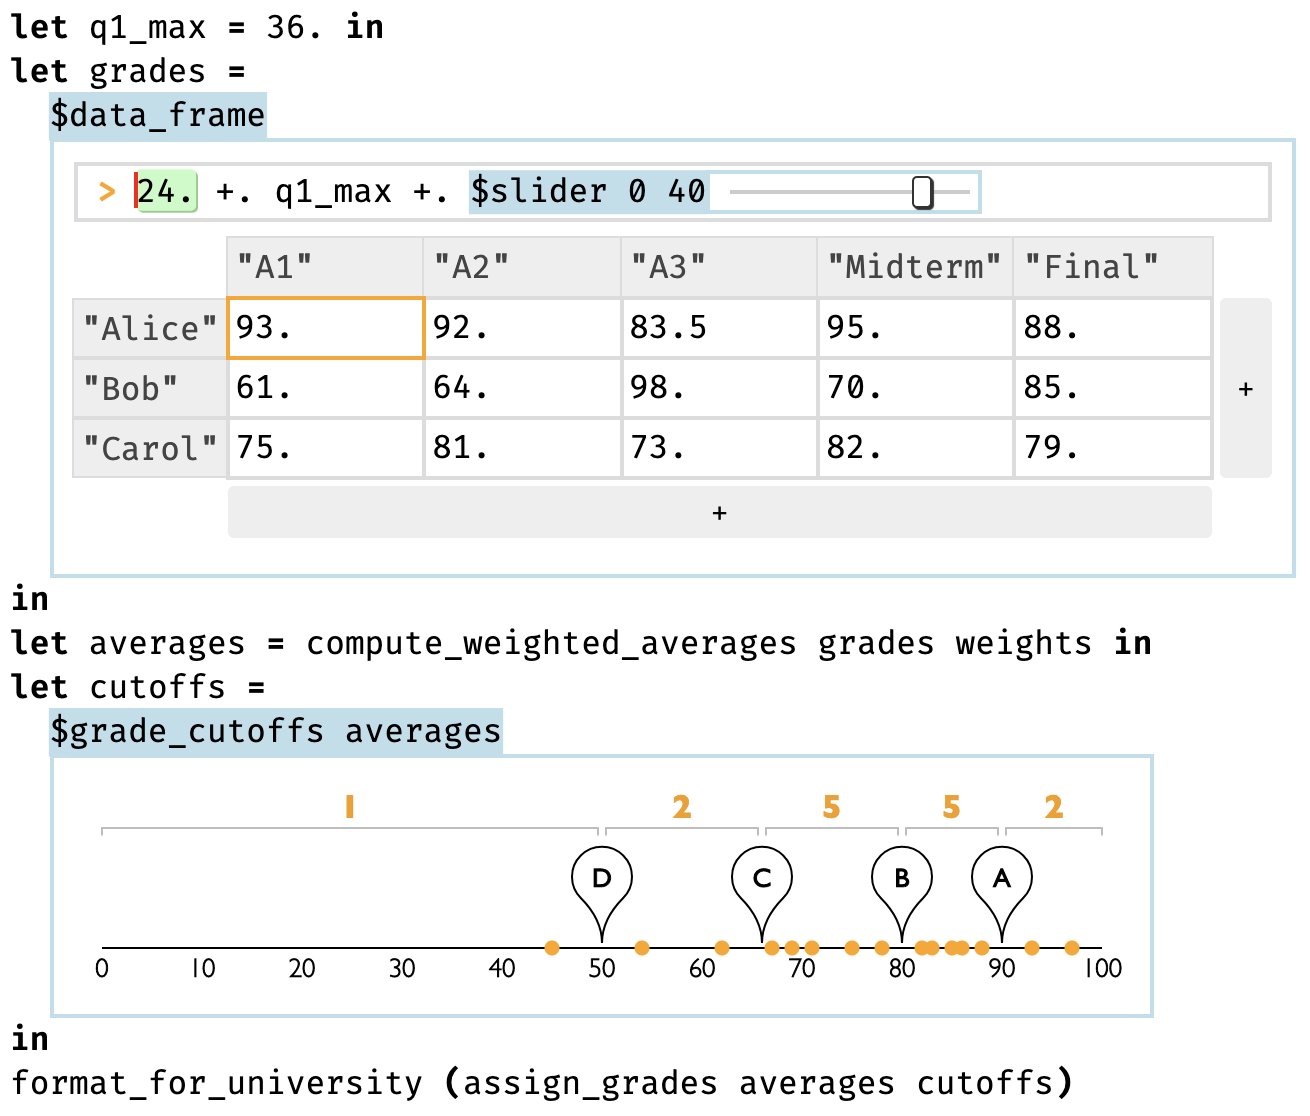
\includegraphics[width=\linewidth]{grade-cutoff-livelit.png}
  \end{subfigure}
  \vspace{-4mm}
   \caption{Introductory Examples}
%   \vspace*{-2mm}
\end{figure*}

We are not the first to integrate GUIs 
into programming.
% Prior work on projectional editing
% and active code completion, detailed in Sec. \ref{sec:related-work},
% has also considered the problem of entering expressions
% of certain types, like \li{Color},
% using specialized GUIs integrated into a program editor.
% We detail prior work in Sec.~\ref{sec:related-work}, but 
The prior work most relevant to this paper is the {Graphite} system for Eclipse for Java,
demonstrated in Fig.~\ref{fig:graphite} \cite{Graphite}.
Graphite allows a library provider to associate a GUI, called a \emph{palette}, with a type 
(via a Java class annotation), here \li{Color}.
Wherever an expression of this type is needed,
i.e. wherever there is a \emph{hole} of this type 
(as determined by Eclipse's online parser and typechecker),
the environment offers the client the option, via the code completion menu,
to generate it using the palette.
Once the user presses \li{Enter} to indicate that the 
interaction is finished, the palette generates a
Java expression to fill the hole, here \li{new Color(57, 107, 57, 235)}.
Several other systems, such as the  
\textbf{mage} system for Jupyter notebooks \cite{DBLP:conf/uist/KeryRHMWP20}
behave analagously.
Projectional editing, the visual macro system in Racket \cite{interactive-visual-syntax}, and a number of other designs
also confront this general problem of integrating GUIs with symbolic code
in broadly similar ways.

\citet{Graphite} evaluated Graphite by surveying 473 developers 
and \citet{DBLP:conf/uist/KeryRHMWP20} evaluated \textbf{mage} by interviewing 9 developers.
Both studies found that
participants viewed the proposed mechanism favorably and 
would use a suitable GUI some or all of the time.
% \footnote{When presented with a color palette,
% many participants remarked that they rarely entered colors directly into Java code,
% but rather into stylesheets.
% Other palettes, e.g. a palette
% that supported regular expression construction, were viewed as more
% suitable for Java code.
% The mechanisms being considered are suitable both for general-purpose languages
% and typed domain-specific languages like typed stylesheets, which can often be embedded into modern
% general-purpose languages.}
This and other prior work also collectively showcase a wide variety of use cases \cite{Graphite,DBLP:conf/uist/KeryRHMWP20,interactive-visual-syntax}, 
and the Graphite survey solicited dozens of additional use cases from participants,
which the authors systematically taxonomize \cite{Graphite}. 
We take these extensive empirical findings   
as evidence for, and a showcase of, 
the value of this broad class of mechanisms for integrating GUIs with code.
\vspace{-1mm}
\subsection{Contributions}
\label{sec:contributions}
We turn our attention in this paper to a number of fundamental technical
deficiencies that limit both GUI providers and clients using these prior mechanisms.
To address these, 
we introduce a system of \emph{live literals}, or \emph{livelits}, 
demonstrated in Fig.~\ref{fig:color}. 
Livelits are unique in achieving all of the following properties.
(Sec.~\ref{sec:related-work} describes which subset of these  
are achieved by prior systems,
including those just mentioned.)

\newcommand{\llproperty}[1]{\vspace{5px}\noindent\textbf{#1}.}

\llproperty{Decentralized Extensibility}
    Providers define livelits in libraries. 
    Clients invoke livelits by name. Livelit names, e.g. \li{\$color}, 
    are prefixed by \li{\$} (pronounced ``lit''),    
    to distinguish them from variables.
    We call this \emph{decentralized extensibility}
    to distinguish it from systems that are not extensible or 
    that can only be extended via editor extensions or editor generation.
    % Both mage and Racket's visual syntax system are similarly extensible, 
    % but 
    % In Graphite, palettes are associated with class definitions, 
    % so there is a tighter association between 
    % as distinct from systems that 
    % are either non-extensible or cannot be extended by library providers.
 
\llproperty{Persistence}
  % In Graphite and \textbf{mage}, GUIs are {ephemeral},
  % i.e. they disappear after the initial interaction,
  % leaving behind only the generated textual code.
  % Only the programmer that initially enters the expression
  % benefits from the feedback and affordances that the GUI provides.
  % %
  % \footnote{Graphite does include an \emph{ad hoc} mechanism that
  % allows palettes to parse the code that is selected in the editor
  % when the palette loads, but this requires that each palette implement
  % a parser for the subset of Java used in the code that it generates,
  % and therefore this mechanism is quite brittle. It is also difficult
  % to persist GUI state that is not included in the generated code.}
  Livelit invocations are expressions, i.e. they  are persistent elements of the syntax tree. They operate as  
  graphical literals, rather than as the ephemeral code generation GUIs of Graphite and \textbf{mage}. 
  We define a pure model-view-update-expand architecture
  (a variation on Elm's model-view-update architecture \cite{ElmArchitecture}) 
  where only the model needs to be persisted.
  The dynamic meaning of a livelit is determined by a macro expansion step.
  % We chose the word ``literal'' rather than ``palette'' because,  persistence, livelits
  % operate as graphical literals.

\llproperty{Compositionality}
% Prior systems have limited or no support for {entering sub-expressions within the GUI}, 
% so they are useful mainly for generating expressions composed of constants,
% e.g. color constants in Fig.~\ref{fig:color}(a).
%
   Livelit GUIs can embed sub-expressions, which we call \emph{splices} (after
   \citet{TLMs}).
  Fig.~\ref{fig:color} demonstrates splicing: the RGBA components  
  are each splice editors, so the client can define a variable, \li{baseline},
  to relate the color components (here, to explore greens by offsetting the green component past the baseline)
  and use a slider livelit inline to specify the alpha component.
  % Similarly, Fig.~\ref{fig:grading}(b)\todo{subfigure labels}{} demonstrates a 
  %  data table livelit where each entry is a splice.
  
  Crucially, composition is  
  governed by a binding discipline that ensures 
  (1) \textbf{capture avoidance}, i.e. that variables that the client uses in splices, like \li{baseline},  
  are lexically scoped to the livelit invocation site (so they cannot inadvertently capture expansion-internal bindings, which can therefore be left abstract); and 
  (2) \textbf{context independence}, i.e. that the livelit 
  can be invoked and operate in any lexical context (so the client need not worry about naming conflicts or manage hidden library dependencies).
  This binding discipline is a form of ``macro hygiene'' \cite{TLMs, adamsHygiene, DBLP:conf/popl/ClingerR91}, 
  though note that we take a particularly restrictive approach to hygiene compared to, for example, the Racket macro system \cite{DBLP:conf/popl/Flatt16}: 
  new binding and control flow constructs intentionally cannot be expressed to allow clients to understand splices as   
  function parameters (and indeed this is how they are internally handled).

 %without pre-condition or conflict.

\llproperty{Parameterization} Livelits can also take parameters directly, forming parameterized families.
  For example, \li{\$slider} in Fig.~\ref{fig:color} is parameterized by the slider's bounds.
  Parameters operate like splices, differing in that they can be partially applied in
  livelit abbreviations. For example, Fig.~\ref{fig:color}
  partially applies \li{\$slider} to \li{0} and \li{100} to define a \li{\$percent} slider.
  % \begin{lstlisting}[numbers=none]
  % let $percentage = $slider 0 100 in ...
  % \end{lstlisting}
  % Parameterization also underlies the hygiene mechanism, as we will discuss in Sec.~\ref{sec:livelit-definitions}.

\llproperty{Typing} Each livelit must specify an expansion type, 
and parameters and splices must also specify types, 
so livelits are compatible with type-driven development.
Together with the binding discipline, 
this allow clients to reason abstractly, i.e.  
without inspecting the expansion or livelit implementation.
% in the manner of a function application. 

\llproperty{Liveness} Uniquely, livelits can evaluate splices 
  throughout the editing process 
  (i.e. in a \emph{live} manner \cite{DBLP:conf/icse/Tanimoto13}) 
  to provide feedback related to run-time behavior.
  For example, in Fig.~\ref{fig:color}, 
  displaying the selected color requires evaluating the RGBA
  component splices to numeric values.
  Evaluation occurs in a run-time environment (i.e. closure) determined by
  leaving the hole being filled by the livelit temporarily unfilled and then evaluating
  using a two-phased variant of the semantics for 
  Hazelnut Live \cite{HazelnutLive}.
  Live evaluation is supported even for livelits 
  that appear inside a function: multiple function calls 
  can lead 
  to multiple closures that the client 
   selects between.

\paragraph{Outline.} Sec.~\ref{sec:case-studies} introduces
livelits from the perspective of client programmers. 
% Our examples are organized into case studies 
% that demonstrate the novel contributions of this paper.
Sec.~\ref{sec:livelit-definitions} then 
considers the livelit provider's perspective by introducing livelit
definitions with a detailed example.
Sec.~\ref{sec:livelit-calculus} defines the \emph{typed livelit calculus}. 
We have mechanically specified the central mechanism, livelit expansion, 
and proven the associated metatheorems in Agda.
This calculus 
serves to capture the essential nature of livelits 
independent of the particularities of syntax, GUI frameworks, 
and other orthogonal design details,
because we believe livelits can be integrated into a wide variety of programming systems. 
Sec.~\ref{sec:implementation} provides a more detailed account of our implementation of livelits.
Our primary implementation, used in the screenshots in the paper,
is integrated into Hazel, a live functional programming environment designed 
around hole-driven development. 
We have also prototyped livelit editing within a standard text editor. 
Additionally, we discuss factors that must be considered when integrating livelits into languages with side effects.
Sec.~\ref{sec:related-work} compares livelits to related work using the design properties outlined above 
as a rubric.
We conclude in Sec.~\ref{sec:discussion} after a discussion of present limitations and several directions for future work.